

\documentclass[a4paper,11pt]{article} 
\usepackage[spanish]{babel}           
\usepackage[utf8]{inputenc}           

\usepackage[T1]{fontenc}   		   % Fonte por defecto.
\usepackage{graphicx, subfigure}    		   % Engadir imaxes.
\usepackage{color}      		   % Uso de cores.
\usepackage{anysize}     		   % Modificar o tamaño dos marxes.
\usepackage{multicol, multirow}    % Escribir a doble, triple...columna.
\usepackage{bm}          		   % Letras gregas en negriña.
\usepackage{textcomp}    		   % Símbolos, poden consultarse na rede.
\usepackage{eurosym}     		   % Símbolo € (\euro).
\usepackage{amsthm}                % Paquete da AMS para escribir teoremas.
\usepackage{amsmath,amsfonts}      %Paquetes específicos de símbolos.
\usepackage{lineno}                % Numerar as liñas. 

\marginsize{1.5cm}{1.5cm}{1.5cm}{1.5cm} % MARXES: Esq, der, sup, inf.
\parindent=0mm                        % Sangría. 
\parskip=2mm                          % Espazo entre párrafos.
\renewcommand{\baselinestretch}{1}    % Interliñado.
\renewcommand{\spanishtablename}{Táboa} 


\title{Tema 1: Introducción ó estudo da memoria humana}
\date{}


\begin{document}  

\maketitle 

\section{Necesidade e importancia da memoria}
A memoria ten valor adaptativo, posto que está implicada en estratexias evolutivas de adaptación. Ademais das respostas adaptativas que veñen xeneticamente programadas nos organismos, estes son capaces de adaptarse ó seu medio grazas ós procesos de aprendizaxe e memoria.

En canto á nosa especie, a función primaria da memoria humana é dotar ós individuos do coñecemento necesario para guiar unha conduta adaptativa, independentemente da complexidade da situación.

Por outra banda, a memoria está relacionada con outros procesos cognitivos. A súa presenza é clave para o funcionamento de tareas moi variadas (recordo, recoñecemento, aforro de tempo, habilidades...). Porén, non sempre funciona correctamente, e poden producirse erros. Algúns deles englóbanse no que Freud denominou ``psicopatoloxía da vida cotiá'', e outros poden indicar a existencia dun síndrome amnésico.

A memoria ten un papel central na cognición, en tanto que participa en tódolos procesos básicos:

\begin{itemize}
	\item[-] A \textbf{percepción} non é só unha recepción de estímulos, senon unha construción de 			coñecemento que se leva a cabo grazas ós datos previos que almacenamos na memoria. 
	\item[-] A \textbf{atención} dirixe o noso interese cara aqueles puntos onde, grazas á 					experiencia na memoria, cremos que haberá información relevante.
	\item[-] Os procesos de \textbf{pensamento} e \textbf{linguaxe} semellan depender en gran medida 		da información previa e da representación desta na memoria. 
	\item[-] En xeral, a \textbf{aprendizaxe} é un proceso estreitamente vinculado á memoria.
\end{itemize}

\section{Aproximación histórica}
\begin{itemize}
	\item \underline{Alemaña, século XIX}: Ebbinghaus é o primeiro en demostrar que se pode estudar a 	memoria experimentalmente. Máis tarde, a súa tradición desenvólvese principalmente nos EEUU, no 		que se denomina o ``Enfoque da aprendizaxe verbal''.
	\item \underline{EEUU, 1930-1960}: O enfoque da aprendizaxe verbal céntrase nas asociacións 			observables estímulo-resposta, e dedica moito tempo a caracterizar como memorizan os individuos e 	se recordan palabras (reais e sen sentido). A investigación céntrase máis en documentar os 				fenómenos que en explicalos.
	\item \underline{Alemaña e Norte América, 1930}: Aparece a psicoloxía da Gestalt, co que se 			despraza a énfase da conduta cara 	as representacións internas, destacando o papel activo do 			individuo que aprende e recorda.
	\item \underline{Gran Bretaña, 1930}: Bartlett destaca os complexos aspectos sociais da memoria, 		incluíndo os esquemas (representacións internas e culturais sobre o mundo que poden conducir a 			erros na memoria). Rexeita a aprendizaxe de mateterial sen significado como método para o estudo 		da memoria.
	\item \underline{Gran Bretaña, 1950-1960}: Aparece o ``Enfoque do procesamento da información''. 		Empregando a metáfora do ordenador, podería considerarse que a memoria humana comprende un ou 			máis sistemas de almacenamento. Este enfoque inspira o nacemento da Psicoloxía Cognitiva.
\end{itemize}

\subsection{A tradición de Ebbinghaus}
Destacamos unha serie de características:
\begin{enumerate}
	\item Aplica, por primeira vez, o método experimental ó estudo da memoria.
	\item No marco teórico do asociacionismo, estuda a memoria na súa forma ``pura'', como función da 	aprendizaxe.
	\item Promove a simplificación e o control experimental. Estuda os factores que rixen a 				aprendizaxe repetitiva e a retención de material moi sinxelo, baixo condicións moi controladas. 
	\item Desenvolve a ``Tarefa de reaprendizaxe e método dos aforros'', que serve para estimar a 			cantidade de material retido medindo a dificultade de reaprendelo. O material empregado é un 			conxunto de sílabas illadas sen sentido, constituídas por secuencias CVC.
	\item Mide a tasa de aprendizaxe segundo dous principios:
	\begin{itemize}
		\item[-] A Hipótese do tempo total, que establece unha relación lineal entre a práctica e a 			aprendizaxe.
		\item[-] O Efecto da distribución da práctica, segundo o cal a práctica distribuída é máis 				efectiva (isto é, provoca unha maior aprendizaxe) que a práctica masiva.
	\end{itemize}
	\item Mide a tasa de olvido a través dunha relación logarítmica.
\end{enumerate}

Ebbinghaus demostra que un problema complexo e aparentemente inabordable pode estudarse de forma experimental. Porén, obvia a gran riqueza e complexidade da memoria na vida cotiá nos seus estudos.

\subsection{A tradición de Bartlett}
Bartlett publica o seu libro \textit{Remembering} en 1932. Nesta obra critica a Ebbinghaus por excluír o significado nos seus estudos, argumentando que o estudo da aprendizaxe de sílabas sen sentido só revela o funcionamento dos hábitos repetitivos. Sostén que a tradición de Ebbinghaus se limita demasiado ó estímulo, ignorando as actitudes do suxeito e os seus coñecementos previos e supoñendo que un estímulo pobre pode producir unha situación de aprendizaxe sinxela, cando o esforzo por atopar un sentido ó que se aprende é clave para a aprendizaxe humana.

Así, Bartlett propón que aínda que o material con significado sexa máis complexo, tamén é posible estudalo no laboratorio. Os seus experimentos baséanse na utilización de material complexo, como contos populares doutras culturas, e os métodos que emprega son a reprodución repetida e a reprodución serial.

Un dos relatos que emprega máis frecuentemente é \textit{A guerra dos fantasmas}, que por ser doutra cultura é de difícil comprensión e recordo para os suxeitos. Por este motivo obtén a miúdo resultados pouco coherentes, omisións e reconstruccións distorsionadas.

O traballo de Bartlett inclúese na tradición cognitivista europea. A súa teoría considérase vaga e de pobre metodoloxía. Porén, serve de influencia para a moderna teoría dos esquemas e aporta maior validez ecolóxica ó estudo da memoria.

\subsection{Influencia da metáfora do ordenador}
Ó empregar o ordenador dixital como metáfora, a memoria humana podería considerarse como un conxunto dun ou varios sistemas de almacenamento. Calquera sistema de memoria require	tres capacidades: a de \textit{codificar} ou agregar información ó sistema, a de \textit{almacenala} e a de atopar e \textit{recuperar} a información. Aínda que teñen funcións distintas, estas tres fases interactúan entre elas de forma complexa, xa que a nosa memoria comprende varios sistemas de memoria relacionados entre si.

\begin{figure}[h!]
	\centering
	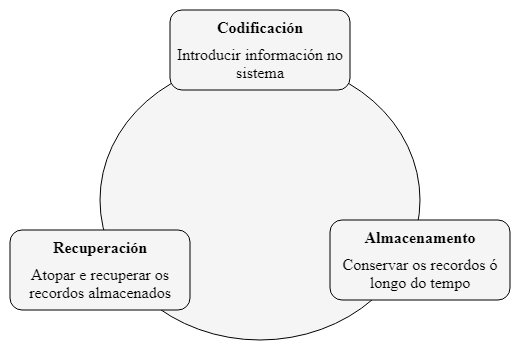
\includegraphics[width=0.65\linewidth]{memoria1_1}
\end{figure}

\section{Modelo modal e sistemas de memoria}
\begin{figure}[h!]
	\centering
	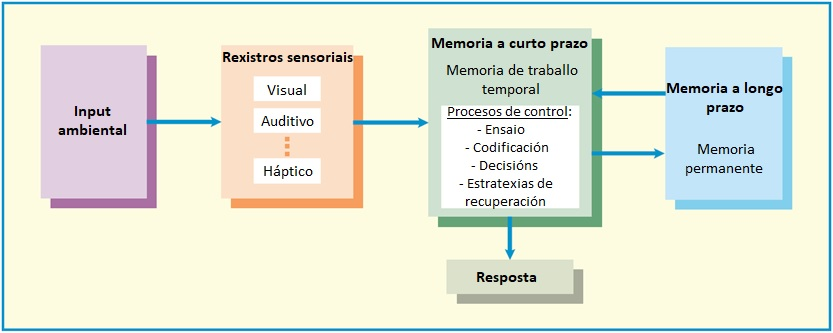
\includegraphics[width=0.95\linewidth]{memoria1_2}
	\caption{Fluxo de información a través dos sistemas de memoria segundo o modelo modal de Atkinson 	e Shiffrin (1968)}
\end{figure}

Este modelo é ampliamente aceptado ó longo dos anos setenta. Propón que a información ambiental se procesa grazas a unha serie de sistemas de memoria sensorial, que poderían considerarse unha especie de interface entre a percepción e a memoria. A información pasa logo a un sistema de memoria temporal, a curto prazo, antes de ser rexistrada na memoria a longo prazo.

Hoxe en día mantéñense as subdivisións de memoria plantexadas no modelo, porque nos axudan a comprender como esta está organizada no noso cerebro. Porén, descártase a idea de que só existe un fluxo de información procedente do ambiente e dirixido á memoria a longo prazo. Os datos de diversas investigacións suxiren que a información se move en ambas direccións. 

\section{Memoria sensorial}
Este tipo de memoria permite a persistencia temporal dun estímulo máis alá da súa presenza física, para que poida ser percibido. Este mecanismo realiza un rexistro precategorial de gran capacidade e curta duración.

Os antecedentes do estudo da memoria sensorial atopámolos no modelo de Broadbent (1958), que é o primeiro en suxerir un mecanismo de memoria inmediata que rexistra toda a información do input sensorial durante un breve periodo de tempo.

Falaremos de dous tipos de memoria sensorial: a memoria icónica e a memoria ecoica.

\subsection{Memoria icónica: O paradigma do informe parcial}
Sperling estuda a memoria sensorial empregando estímulos visuais. O seu obxectivo é o de determinar a cantidade de información dispoñible para un observador despois dunha breve exposición visual. Comeza entón o estudo da \textbf{amplitude de aprehensión}, isto é, o maior número de ítems que poden lembrarse inmediatamente despois dunha breve exposición visual. En 1960 publica ``A información dispoñible en presentacións visuais breves'', resumo da súa tese doutoral.

Os ensaios consisten en presentacións moi breves de series de 12 letras, organizadas en matrices $3*4$. Tras cada presentación pide ós participantes que lembren as letras presentadas, obtendo que estes, en xeral, só son quen de sinalar correctamente catro ou cinco ítems. Isto é o que se denomina \textbf{condición de informe total}, aquela na que se pide informar dunha exposición visual completa.

Ante estes resultados, Sperling facilita un pouco o experimento reducindo o número de ítems a recordar. Establece a \textbf{condición de informe parcial}, na que só se pide informar dunha porción aleatoria da exposición estimular completa. Así, sinala cun tono (agudo, medio ou grave) a fila de letras da matriz que os participantes deben lembrar (primeira, segunda ou terceira, respectivamente).  

\begin{figure}[h!]
	\centering
	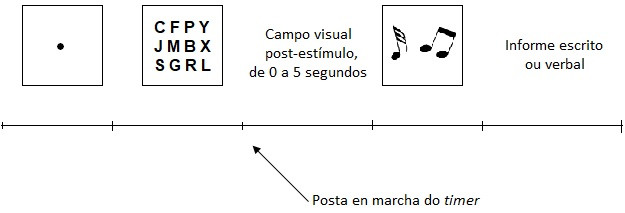
\includegraphics[width=0.8\linewidth]{memoria1_3}
	\caption{Diagrama esquetático dun ensaio estándar nos experimentos de Sperling (1960)}
\end{figure}

Sperling interpreta os seus datos concluíndo que as letras son transmitidas dun almacén visual periférico a outro máis duradeiro, chamado buffer de recoñecemento, a un ritmo de unha cada 10 ms. Supón que este buffer retén a información o tempo suficiente como para poder informar sobre ela. 

Con este experimento confírmase que a cantidade de información dispoñible no instante inmediato á presentación do estímulo breve é superior á amplitude de aprehensión do suxeito. Polo tanto, o que determina esta amplitude non son os límites do sistema perceptivo, senon o tempo necesario para informar dos ítems vistos.

Máis tarde, na súa reinterpretación deste traballo, Neisser propón o termo ``memoria icónica'' para designar o inicial e breve almaceamento visual.


\subsubsection{A curva do olvido da memoria icónica}
Ó longo do experimento, Sperling decide manipular o intervalo temporal entre a desaparición do estímulo visual (matriz de letras) e o sinal auditivo que sinala a fila a informar. Decátase de que a medida que aumenta a demora do sinal prodúcese un deterioro no recordo das letras. Cun segundo de demora, os resultados son comparables ós do informe total (entre 4 e 5 ítems lembrados).

\begin{figure}[h!]
	\centering
	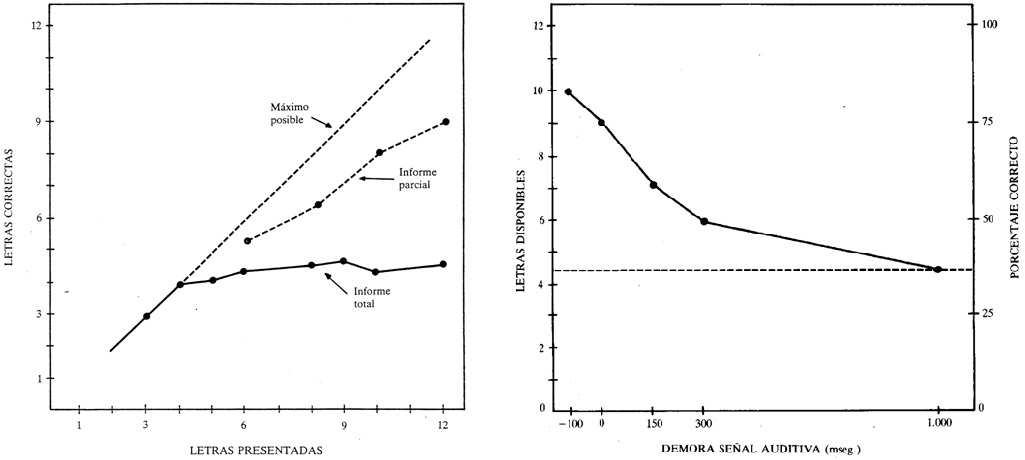
\includegraphics[width=0.98\linewidth]{memoria1_4}
\end{figure}

\subsection{Memoria ecoica}
O nome proposto por Neisser para designar ó equivalente auditivo da memoria icónica é o de ``memoria ecoica''. Falamos dun sistema precategorial, de gran capacidade e persistencia limitada que retén literalmente a información do input antes de que sexa procesada. Esta memoria leva a cabo un rexistro análogo ó da icónica, pero posúe propiedades específicas: retén as propiedades temporais da información, non as espaciais. Isto débese a que a información auditiva é secuancial (fala, música, etc.). 

Un clásico estudo de memoria ecoica é o de Darwin, Turvey e Crowder (1972), a través da técnica do informe parcial. Este experimento coñécese como ``Procedemento do home dos tres oídos'', e nel preséntanse ó mesmo tempo tres mensaxes auditivas provintes de tres lugares distintos (oído dereito, oído esquerdo e centro, ou ambos oídos). Cada unha destas mensaxes contén tres ítems (dous díxitos e unha letra, ou viceversa) e preséntase a unha velocidade de 3 ítems/s. 

Na condición de informe parcial, o suxeito recibe un índice visual localizado á dereita, esquerda ou centro, en función do son que debe lembrar. A demora na presentación deste índice vai variando sistematicamente (0, 1, 2, 3 ou 4 segundos). Na condición de informe total pídese lembrar a maior cantidade de ítems de tódalas mensaxes. 

Destácanse, sobre este tipo de memoria, dous efectos diferentes:
\begin{itemize}
	\item \underline{Efecto de modalidade}: Recordo inmediato do final da lista (recencia) cando se 		emprega a modalidade auditiva de presentación en lugar da visual. 
	\item \underline{Efecto sufixo}: Deterioro do efecto de recencia debido á presentación dun ítem 		adicional, que o suxeito non ten que lembrar, xusto despois da lista experimental. Un exemplo 			deste efecto obsérvase no estudo de Crowder e Morton (1969), quen postulan a existencia dun 			``almacén acústico precategorial'' que sería a base do efecto de recencia auditiva (pero en 			realidade non se sabe se este efecto se debe máis á memoria ou á percepción).
\end{itemize}

\section{Memoria a curto prazo e memoria de traballo}
\begin{itemize}
	\item \textbf{Memoria a curto prazo (MCP):} Almaceamento de pequenas cantidades de información 			durante breves intervalos temporais (poucos segundos). Inicialmente pensouse que era sobre todo 		verbal, pero hoxe sabemos que pode conter case calquera tipo de material (incluso visoespacial). 		Crese que o repaso emprégase a miudo para conservar ítems na MCP. 
	\item \textbf{Memoria de traballo (MT):} Espazo de traballo mental, vinculado á atención, no que 		a información se mantén temporalmente para a súa manipulación. É útil na realización de tarefas 		complexas e crese que serve de base para o pensamento. Pode empregar recursos propios das 				memorias a curto e longo prazo.
\end{itemize}
 
\section{Memoria a longo prazo}
É o sistema (ou conxunto deles) que sustenta a capacidade de almacenar información durante longos períodos de tempo. Pode dividirse en varios tipos:
\begin{itemize}
	\item \underline{Memoria explícita ou declarativa}: MLP para feitos e eventos.
	\begin{itemize}
		\item \textbf{Memoria episódica:} Memoria para eventos específicos, que se lembran a través 			do que Tulving denomina ``viaxe mental no tempo''. O recordo permite revivir ditos eventos e 			empregar esta información para planear accións futuras.
		\item \textbf{Memoria semántica:} Memoria para o coñecemento xeral sobre o mundo e a 					sociedade. É de natureza xeral, aínda que en ocasións poida adquirirse de xeito específico. 
	\end{itemize}
	\item \underline{Memoria implícita ou non declarativa}: MLP para información que se reflexa máis 		na execución que no recordo ou recoñecemento explícitos (habilidades motoras, condicionamento 			clásico...).
	\begin{itemize}
		\item \textbf{Priming:} Proceso mediante o cal a presentación dun ítem facilita ou dificulta 			o procesamento dun ítem posterior.
	\end{itemize}
\end{itemize}

\begin{figure}[h!]
	\centering
	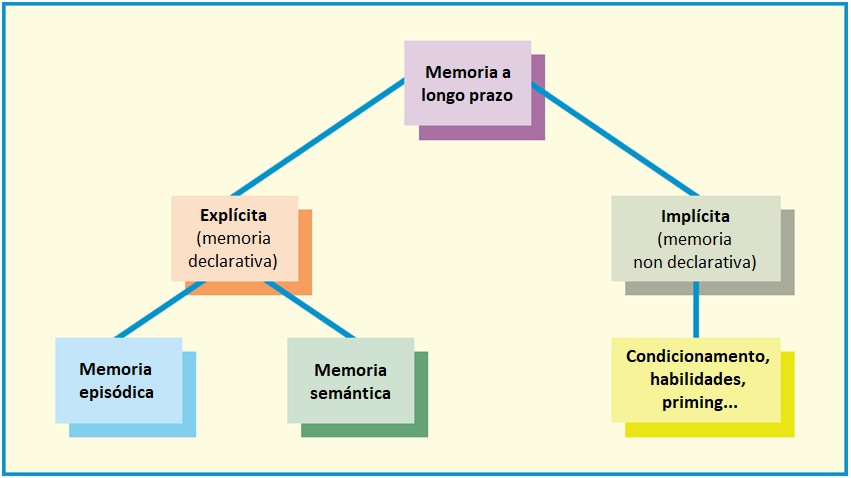
\includegraphics[width=0.9\linewidth]{memoria1_5}
	\caption{Clasificación da memoria a longo prazo proposta por Squire (1992)}
\end{figure}

\subsection{Amnesia}
Unha indicación de que a MLP pode subdividirse en distintos sistemas provén do estudo de pacientes amnésicos. Estes presentan, normalmente:
\begin{itemize}
	\item[-] Deterioros significativos na codificación/recuperación episódica.
	\item[-] Dificultades para formar novas memorias semánticas, o que suxire que estas se forman 			xeralizando información codificada previamente de forma episódica.
	\item[-] Capacidade preservada para adquirir e empregar memorias implícitas. 
\end{itemize}

Isto é, son capaces de aprender pero non de recordar o contexto no que aprenderon, porque olvidan a situación de aprendizaxe.

Un estudo clásico de amnesia é o de Édouard Claparede (1911). Este neurólogo deseñou un experimento que consistía en saudar ós seus pacientes cada vez que chegaba á súa clínica cun apretón de mans. Cando chega o turno de saudar á súa paciente amnésica, agocha un alfiler na palma da man e pínchaa con el.

Ó día seguinte, cando vai saludar a esta paciente, ela non recorda o que sucedeu o día anterior. Porén, négase a darlle a man. Deste xeito, Claparede descobre o traballo de dous mecanismos de memoria:
\begin{itemize}
	\item[•] Un que intervén na formación de recordos de experiencias, e que os mantén dispoñibles 			para unha posterior evocación consciente (ou explícita).
	\item[•] Outro que funciona fóra da consciencia, controlando a conduta sen coñecemento explícito 		da aprendizaxe pasada (memoria emocional implícita). 
\end{itemize}

Cara finais dos anos 60 tamén se atopa unha evidencia clara do efecto priming en pacientes amnésicos. Estes pacientes tamén posúen memoria implícita pero non explícita, polo que só poden realizar aquelas tarefas que non requiren unha recuperación consciente de experiencias previas e semellantes.

\newpage

\section{A memoria máis alá do laboratorio: Memoria cotiá}
% Please add the following required packages to your document preamble:
% \usepackage{multirow}
\begin{table}[h!]
\begin{tabular}{c|c|c|}
\cline{2-3}
\multicolumn{1}{l|}{}                                   & \textbf{Investigación no laboratorio}                                                                                      & \textbf{Investigación no mundo real}                                                                                                        \\ \hline
\multicolumn{1}{|c|}{\multirow{2}{*}{\textit{Pros}}}    & Maior control experimental                                                                                                 & \begin{tabular}[c]{@{}c@{}}Valida a teoría probándoa en grupos específicos,\\ mentres axuda a desenvolver probas e tratamentos\end{tabular} \\ \cline{2-3} 
\multicolumn{1}{|c|}{}                                  & \begin{tabular}[c]{@{}c@{}}É máis sinxelo desenvolver e probar\\ rigurosamente as teorías, en rápida sucesión\end{tabular} & \begin{tabular}[c]{@{}c@{}}Destaca as lagoas das teorías actuais e\\ promove o desenvolvemento teórico futuro\end{tabular}                  \\ \hline
\multicolumn{1}{|c|}{\multirow{3}{*}{\textit{Contras}}} & \begin{tabular}[c]{@{}c@{}}Sobrerrepresentación de certas\\ poboacións de participantes\end{tabular}                       & \multirow{3}{*}{\begin{tabular}[c]{@{}c@{}}Menor control experimental e máis\\ variables de confusión\end{tabular}}                         \\ \cline{2-2}
\multicolumn{1}{|c|}{}                                  & Reduce a xeralización dos descubrimentos                                                                                   &                                                                                                                                             \\ \cline{2-2}
\multicolumn{1}{|c|}{}                                  & Menor validez ecolóxica                                                                                                    &                                                                                                                                             \\ \hline
\end{tabular}
\end{table}

\section{Estudos neuropsicolóxicos e aportacións da neurociencia}
\begin{itemize}
	\item \underline{Estudos relacionados con trastornos específicos}: Implica caracterizar os 				déficits e as habilidades conservadas en pacientes con enfermidades específicas, por exemplo 			Alzheimer.
	\item \underline{Estudos de lesións}: Implica perfiles de pacientes con dano cerebral orgánico en 	rexións relativamente focais, coma as lesións do hipocampo de HM. 
	\item \underline{Electrofisioloxía (EEG e ERPs)}: A principios do século XX comezan a empregarse 		electrodos situados no coiro cabeludo para rexistrar os sinais eléctricos das neuronas. As
	características das ondas cerebrais continuas poden axudar a detectar actividade cerebral anormal 
	e diferentes etapas de sono e arousal.
	
	Se se dividen estas ondas en segmentos, chamados potenciais relacionados con eventos (ERPs), cada 
	un dos cales comeza cun evento particular, pódese medir a actividade cerebral evocada pola
	presenza de determinados estímulos (potenciais evocados). 
	\item \underline{Técnicas de neuroimaxe}: Permiten estudar a estrutura e a función do cerebro,
	mediante o seguimento de indicadores da actividade cerebral.
	\begin{itemize}
		\item \textbf{Tomografía por emisión de positróns (PET):} Introdúcese unha substancia
		radioactiva no fluxo sanguíneo e faise un seguimento para comparar a actividade metabólica ou 
		o funcionamento dos neurotransmisores de diferentes rexións cerebrais.
		\item \textbf{Imaxe por resonancia magnética funcional (fMRI):} Mídese, de forma non
		invasiva, o consumo de osíxeno no cerebro a partir da alineación de núcleos atómicos baixo un 
		forte campo magnético. 
		\item \textbf{Magnetoencefalografía (MEG):} Rexístranse, de forma non invasiva, as forzas
		magnéticas xeradas polas neuronas. 
	\end{itemize}
\end{itemize}

\newpage

% Please add the following required packages to your document preamble:
% \usepackage{multirow}
\begin{table}[h!]
\centering
\begin{tabular}{|c|c|c|c|}
\hline
\multicolumn{2}{|c|}{}                                                                                                     & \textit{Pros}                                                                                                                        & \textit{Contras}                                                                                                                                                                                \\ \hline
\multicolumn{2}{|c|}{\textbf{\begin{tabular}[c]{@{}c@{}}Estudos relacionados\\ con trastornos\\ específicos\end{tabular}}} & \begin{tabular}[c]{@{}c@{}}Proporcionan unha ruta directa\\ para avanzar no diagnóstico\\ e tratamento das enfermidades\end{tabular} & \begin{tabular}[c]{@{}c@{}}A miúdo é difícil separar os\\ deterioros de memoria\\ doutros déficits relacionados\\ coa enfermidade\end{tabular}                                                  \\ \hline
\multicolumn{2}{|c|}{\multirow{2}{*}{\textbf{Estudos de lesións}}}                                                         & \multirow{2}{*}{\begin{tabular}[c]{@{}c@{}}Axudan a identificar vínculos\\ causais entre cerebro e conduta\end{tabular}}             & Son casos relativamente raros                                                                                                                                                                   \\ \cline{4-4} 
\multicolumn{2}{|c|}{}                                                                                                     &                                                                                                                                      & \begin{tabular}[c]{@{}c@{}}As lesións case nunca se\\ limitan por completo a\\ unha rexión específica de\\ interese e/ou os déficits dos\\ pacientes non son completamente\\ puros\end{tabular} \\ \hline
\multicolumn{2}{|c|}{\multirow{2}{*}{\textbf{Electrofisioloxía}}}                                                          & \begin{tabular}[c]{@{}c@{}}Resolución temporal\\ de milisegundos\end{tabular}                                                        & \multirow{2}{*}{\begin{tabular}[c]{@{}c@{}}Incapacidade para localizar con\\ precisión a rexión cerebral\\ que xera o sinal rexistrado\end{tabular}}                                            \\ \cline{3-3}
\multicolumn{2}{|c|}{}                                                                                                     & \begin{tabular}[c]{@{}c@{}}Coste relativamente\\ baixo e non invasivo\end{tabular}                                                   &                                                                                                                                                                                                 \\ \hline
\multirow{8}{*}{\textbf{\begin{tabular}[c]{@{}c@{}}Técnicas de\\ neuroimaxe\end{tabular}}}     & \multirow{3}{*}{PET}      & \multirow{3}{*}{}                                                                                                                    & \begin{tabular}[c]{@{}c@{}}Dificultade para separar os\\ rápidoscambios no cerebro\end{tabular}                                                                                                 \\ \cline{4-4} 
                                                                                               &                           &                                                                                                                                      & \begin{tabular}[c]{@{}c@{}}Require a exposición\\ a substanciasradioactivas\end{tabular}                                                                                                        \\ \cline{4-4} 
                                                                                               &                           &                                                                                                                                      & Custosa                                                                                                                                                                                         \\ \cline{2-4} 
                                                                                               & \multirow{2}{*}{fMRI}     & \begin{tabular}[c]{@{}c@{}}Maior resolución espacial\\ e temporal que a PET\end{tabular}                                             & \multirow{2}{*}{Máis custosa que a PET}                                                                                                                                                         \\ \cline{3-3}
                                                                                               &                           & Menos invasiva                                                                                                                       &                                                                                                                                                                                                 \\ \cline{2-4} 
                                                                                               & \multirow{3}{*}{MEG}      & \begin{tabular}[c]{@{}c@{}}Maior resolución temporal\\ que as anteriores\end{tabular}                                                & \multirow{3}{*}{\begin{tabular}[c]{@{}c@{}}Máis custosa que as\\ técnicas anteriores\end{tabular}}                                                                                              \\ \cline{3-3}
                                                                                               &                           & \begin{tabular}[c]{@{}c@{}}Proporciona unha medida\\ directa da actividade cerebral\end{tabular}                                     &                                                                                                                                                                                                 \\ \cline{3-3}
                                                                                               &                           & \begin{tabular}[c]{@{}c@{}}Mellor resolución espacial\\ que os EEG/ERPs\end{tabular}                                                 &                                                                                                                                                                                                 \\ \hline
\end{tabular}
\end{table}





\end{document} %Non pode haber nada escrito despois desta instrución.
